\subsection{Buscar una ley en lex.gal}

Se representa la operación de búsqueda de leyes en la base de datos de lex.gal. En este caso, puede ser que no se devuelvan leyes si no se encuentra ninguna, o bien, se devuelven las leyes encontradas. Esta operación se puede realizar desde las páginas Home y Search del cliente.

\begin{figure}[H]
\centerline{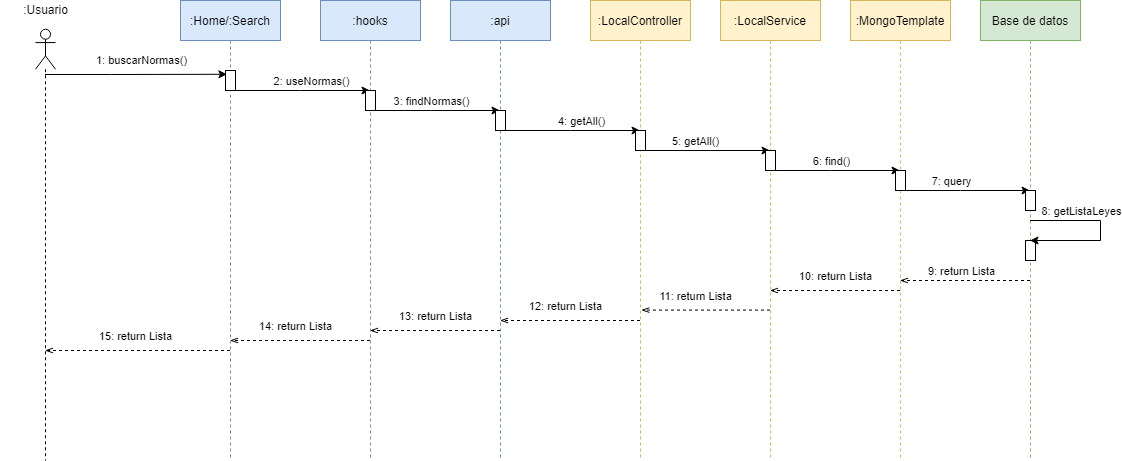
\includegraphics[width=15cm]{figuras/diseño/BuscarLeyLEXGAL.png}}
\caption{Diagrama de secuencia 02. Buscar una ley en lex.gal.}
\label{enlaceDBuscar}
\end{figure}

\begin{enumerate}
    \item El usuario pincha en el buscar leyes en la página de búsqueda, con el texto de sumario si este ha escrito algo, o sin él.
    \item Este método invoca al hook useNormas() del archivo contenido en hooks().
    \item Se invoca al método findNormas() de la carpeta api.
    \item Se hace un llamamiento mediante una solicitud HTTP al servidor. En concreto, la función getAll() de LocalController, pues se hace un GET.
    \item Se invoca al servicio getAll() de FinalDocumentService.
    \item Se invoca la operación find() del template MongoTemplate, pues se busca según un texto, páginas y también tamaño de búsqueda.
    \item Se invoca la operación de recuperar en la base de datos de MongoDB.
    \item Se recuperan las leyes encontradas en la base de datos.
    \item Se procede a devolver la respuesta al usuario desde este paso, realizando el proceso inverso. El usuario recibirá las leyes encontradas de forma paginada, según el texto de sumario que había escrito.
\end{enumerate}